\documentclass[presentation]{subfiles}

\onlyinsubfile{
}
\begin{document}

\section{Complexity}

\begin{frame}{Complexity}
  What do we mean when we talk about complexity?
  % \begin{minipage}[t][25mm][t]{\textwidth}
  %   \begin{columns}
  %     \begin{column}[T]{0.8\textwidth}
        \begin{itemize}
          \item<1->
          Can crowds help you write something?\\
          \scriptsize{\textcite{bernsteinSoylent,Kim:2014:CSI:2556288.2556986,Nebeling:2016:WCW:2858036.2858169}}\normalsize{}
          \item<2-> Can crowds critique novel designs?\\
          \scriptsize{\textcite{yuanAlmost,fuge2014analysis}}\normalsize{}
          \item<3-> Can crowds create things from whole cloth?\\
          \scriptsize{\textcite{KimStoria,Kim2017,Hahn:2016:KAB:2858036.2858364,Lasecki:2014:LSR:2661334.2661352}}\normalsize{}
        \end{itemize}
      % \end{column}
      % \begin{column}[T]{0.2\textwidth}
      %   \begin{figure}
    % \centering
    % \vspace{0mm}

    % \visible<1->{
\includegraphics[width=.33\textwidth]{figures/complexity/geodesic.png}}%
    % \visible<3->{
    % \includegraphics<1->[width=.5\textwidth]{figures/complexity/paper_resized.png}
    %               % 
\includegraphics[width=.33\textwidth]{figures/complexity/chair_resized.png}
    % % }

    % \includegraphics<2->[width=.5\textwidth]{figures/complexity/chair_resized.png}
    
    % 
\includegraphics[width=.15\textwidth]{figures/paper-unfolded.png}$\rightarrow$
    % 
\includegraphics[width=.15\textwidth]{figures/rhino.png}
    % 
\includegraphics[width=.15\textwidth]{figures/fish.png}
    % 
\includegraphics[width=.15\textwidth]{figures/origami-1b.png}
    
    % \vspace{4mm}
    % 
\includegraphics[width=\textwidth]{figures/hexagonflattened.png}
    % \vspace{5mm}
    
    % \visible<2->{
    % 
\includegraphics[width=\textwidth]{figures/complexity/decompose.png}
    % }

    % \visible<4->{
    %   \vspace{5mm}
    %   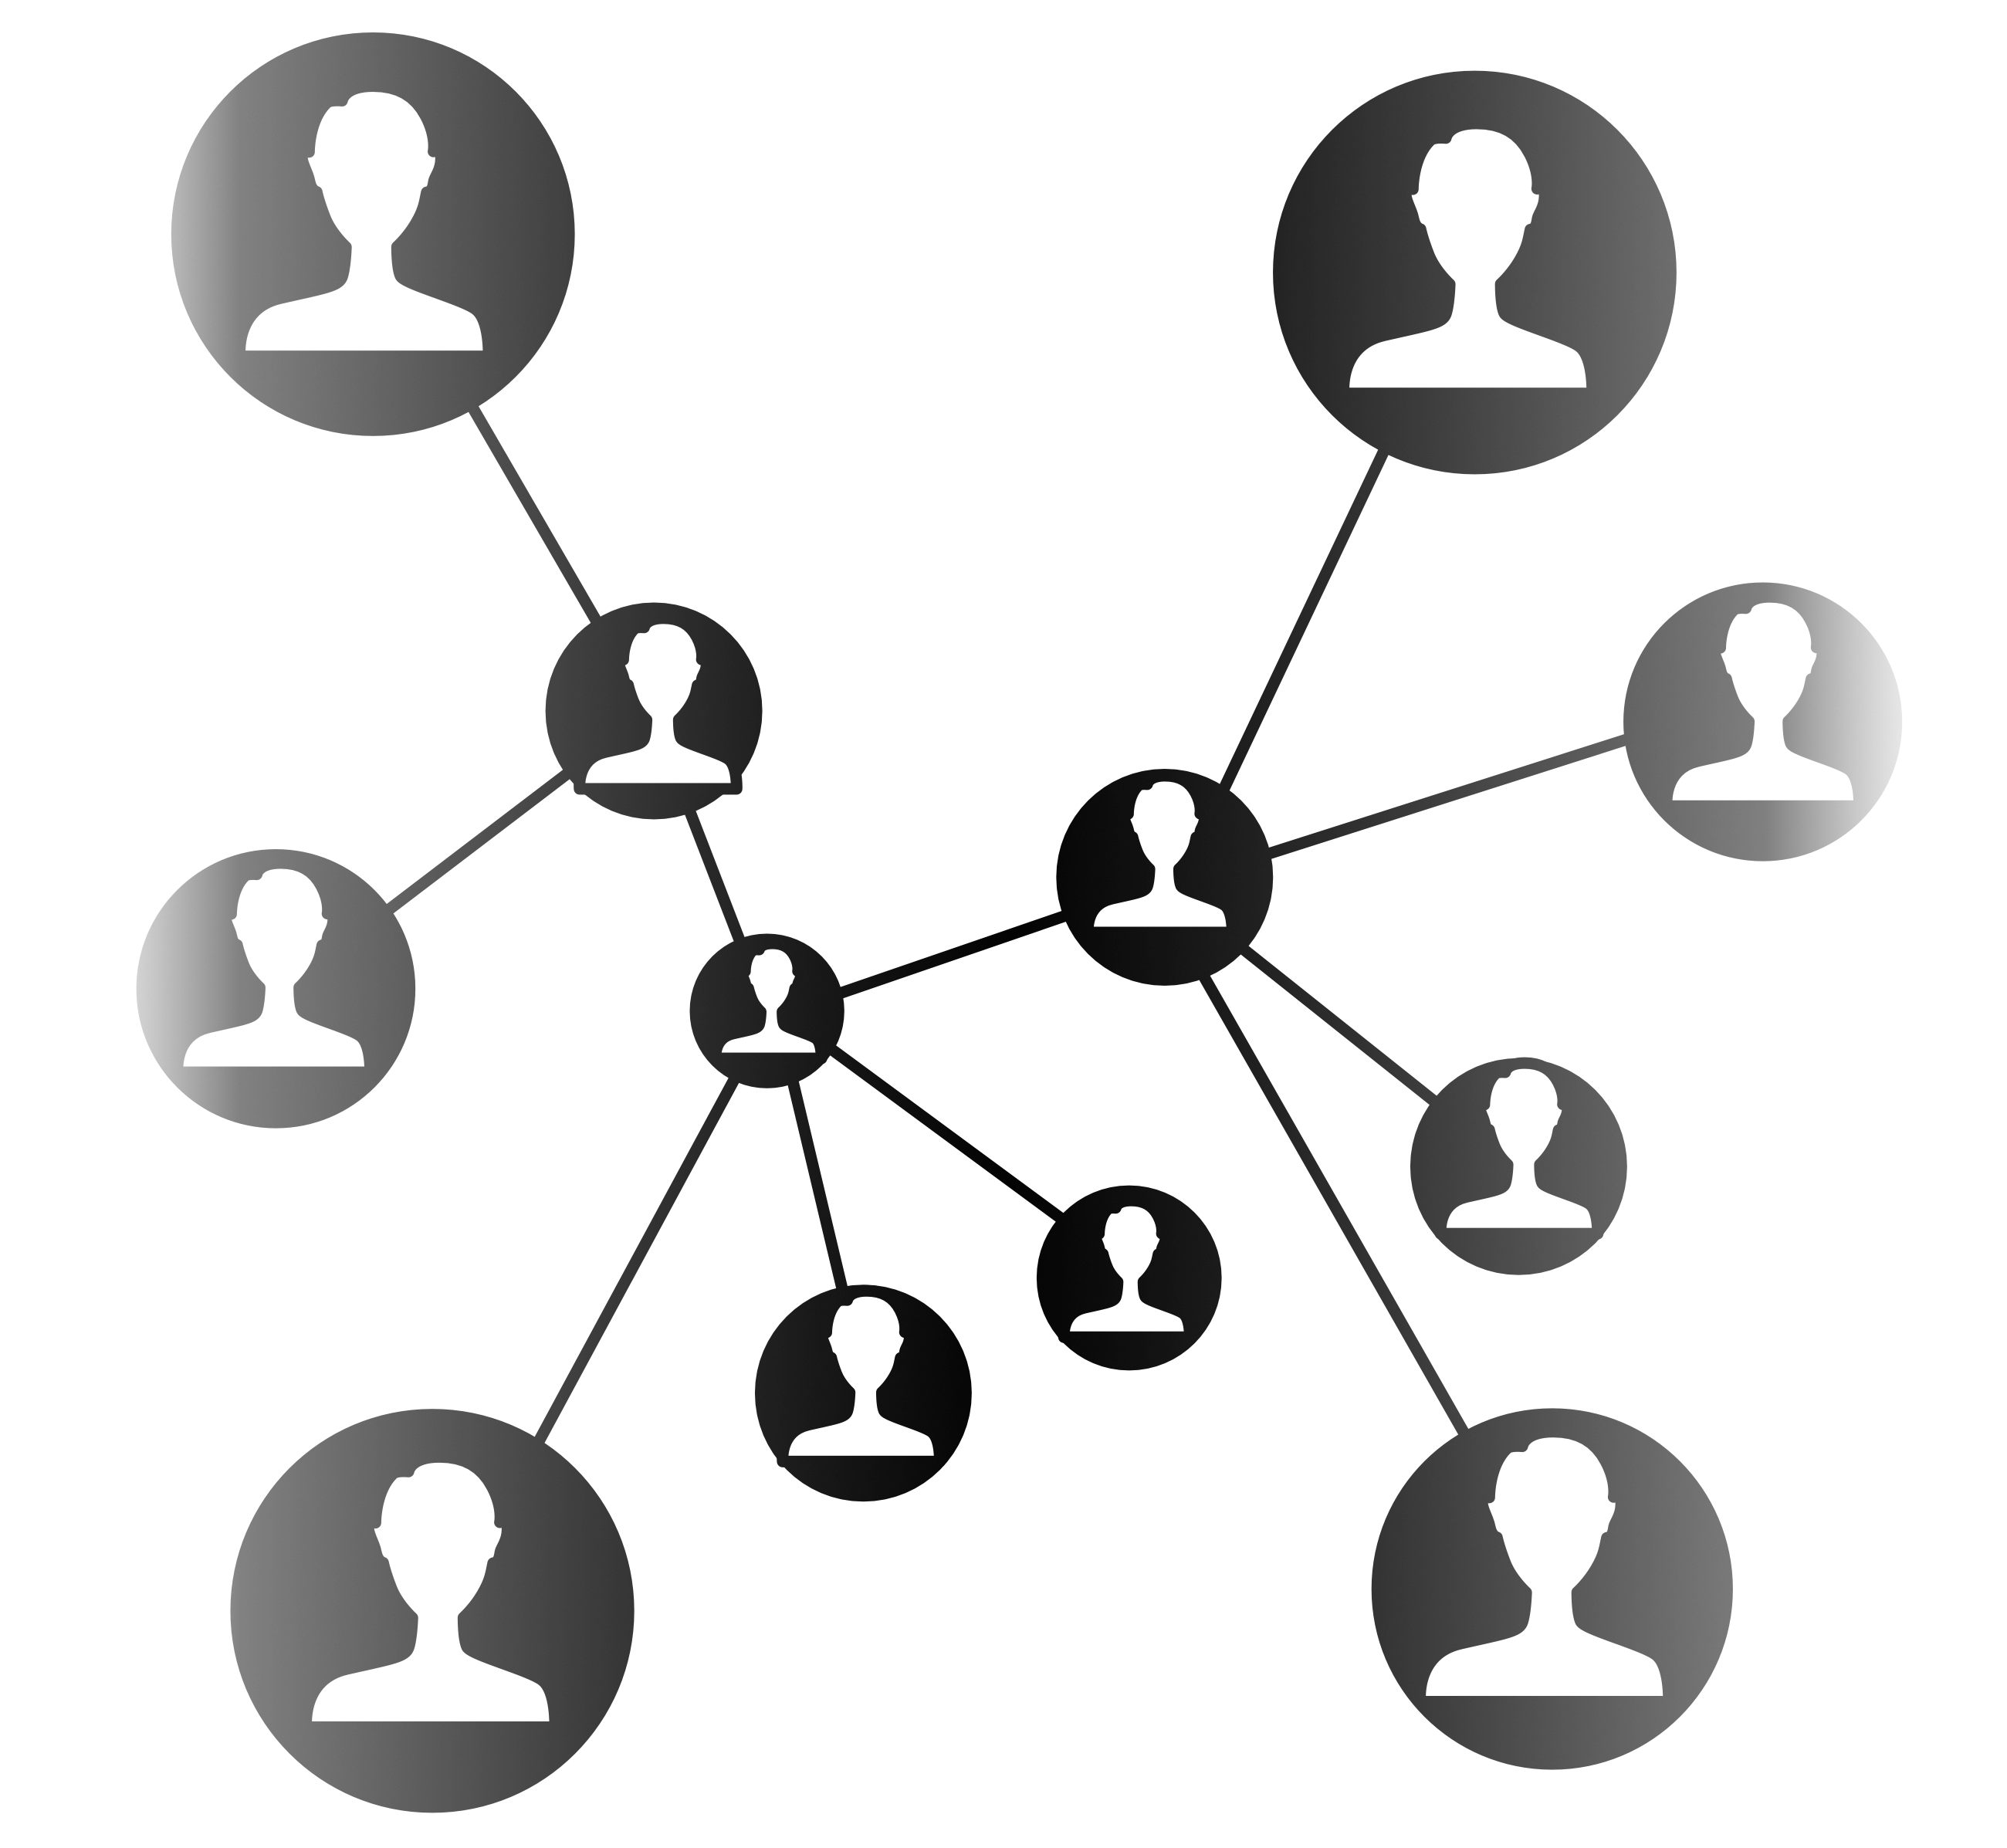
\includegraphics[width=\textwidth]{figures/networkTransparency.png}
    % }
  % \end{figure}
  %     \end{column}
  %   \end{columns}
  %   \end{minipage}
\end{frame}


\begin{frame}{What Does Crowdsourcing Say?}
\begin{columns}
  \begin{column}{0.6\textwidth}
    \begin{itemize}
      \item Build complexity into the process
      \begin{itemize}
        \item<1> Apply CS methods to people\\
        \scriptsize{\textcite{crowdForgeKittur}}\normalsize{}
        \item<2> Humans as computational units\\
        \scriptsize{\textcite{Lasecki:2014:LSR:2661334.2661352}}\normalsize{}
        \item<3> Crowdsourcing workflows as function state machines\\
        \scriptsize{\textcite{latoza2014microtask}
        }
      \end{itemize}
    \end{itemize}
  \end{column}
  
  \begin{column}{0.4\textwidth}
    \begin{figure}
    \only<1>{
    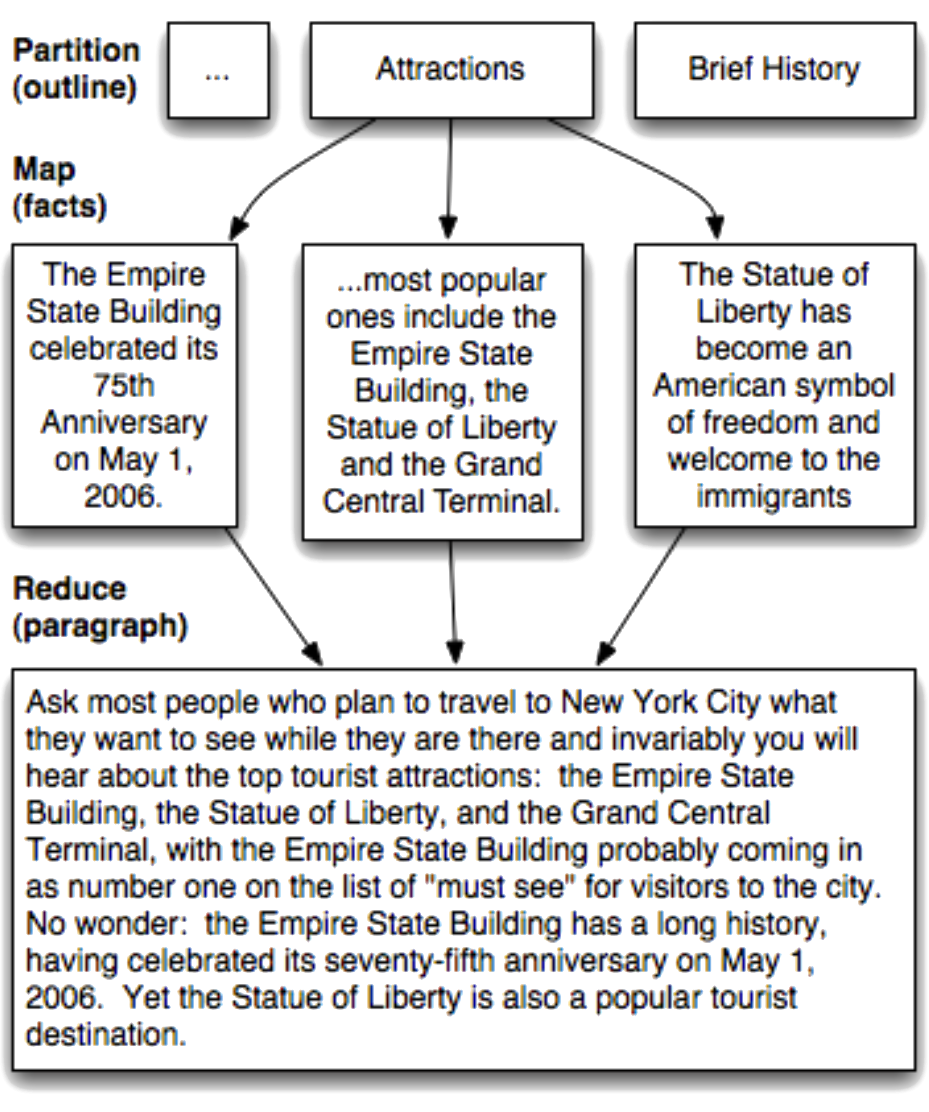
\includegraphics[width=\textwidth]{figures/complexity/cw_literature/mapReduce.png}
    }
    
    \only<2>{
      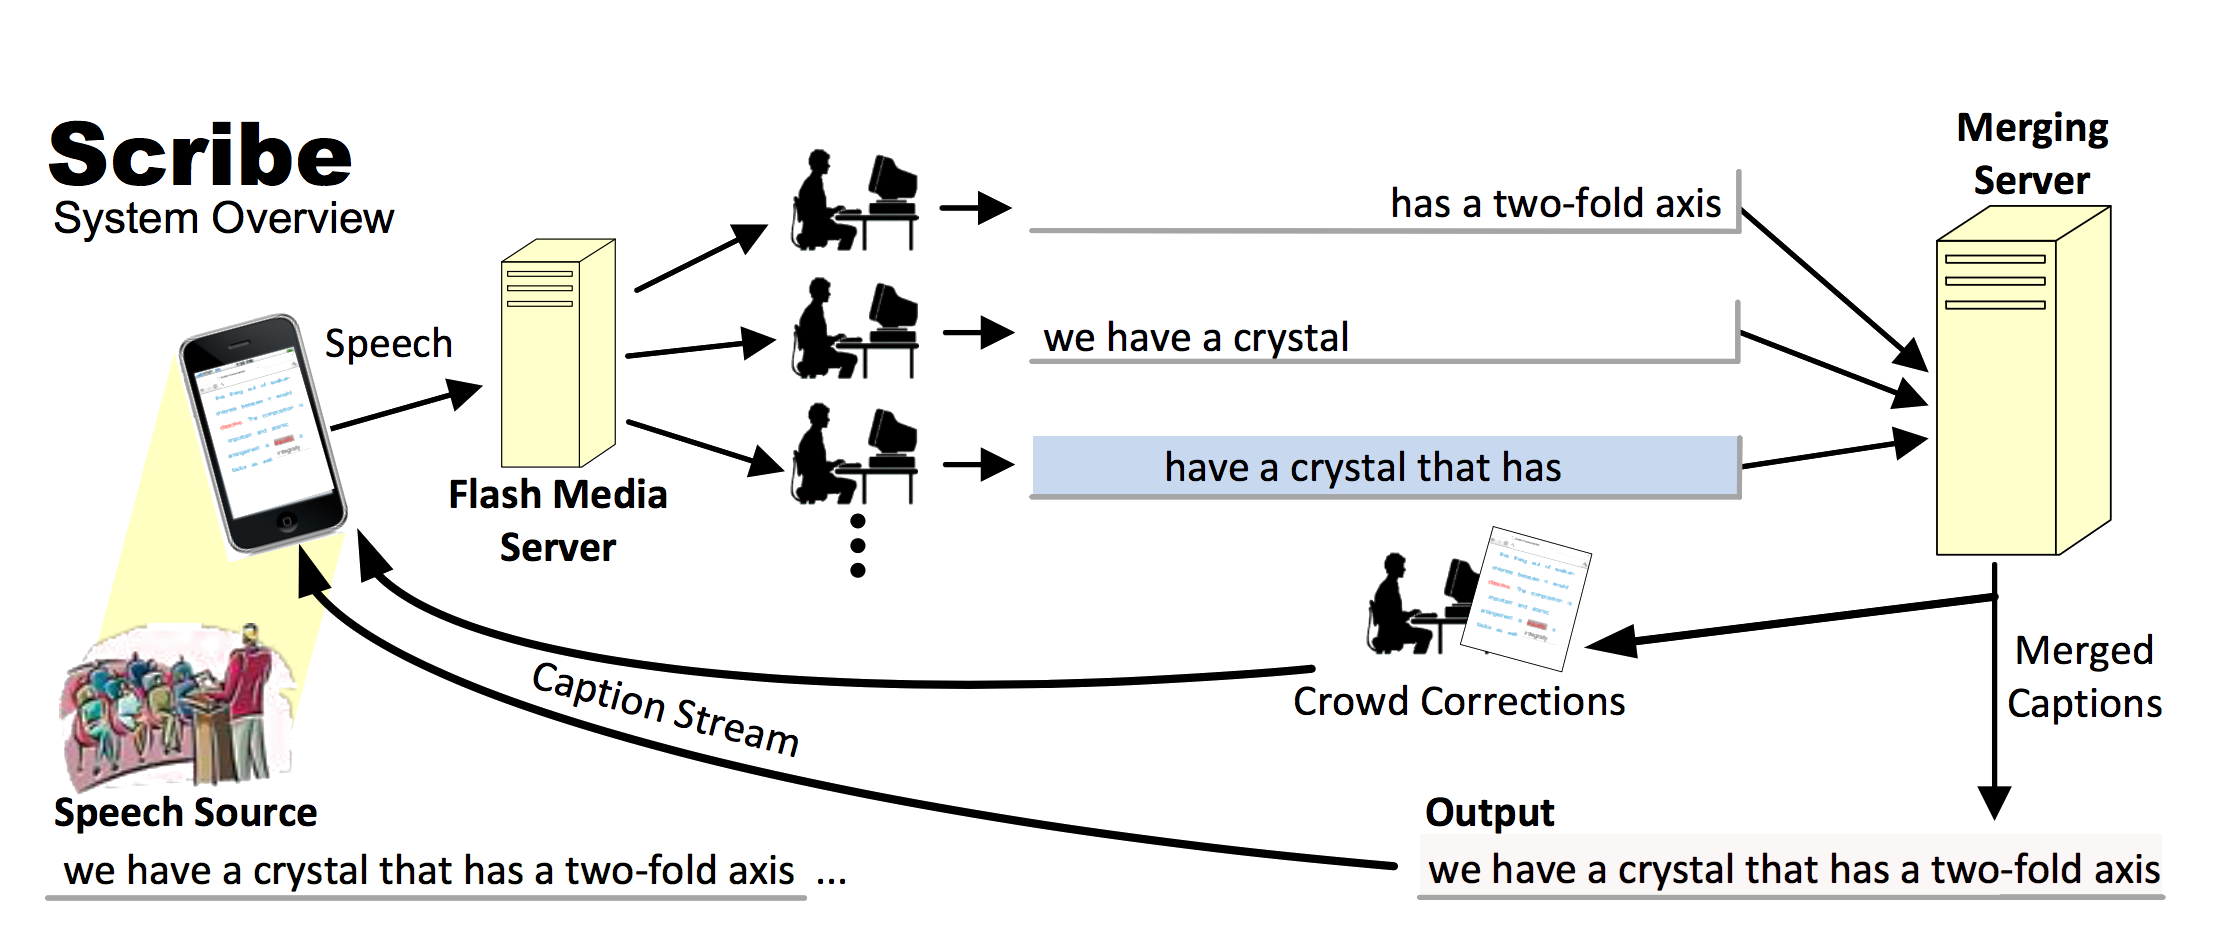
\includegraphics[width=\textwidth]{figures/complexity/cw_literature/scribe.png}
    }
    \only<3>{
      \begin{adjustbox}{max totalsize={\textwidth}{\textheight},center}
      \begin{tikzpicture}[->,>=stealth',auto, node distance=4cm,
                          thick,transform shape]
        \node[state,label=above:{Described}]                       (A)                    {};
        \node[state,label=left:{Described written}]                (B) [below of=A]       {};
        \node[state,label=left:{Run Tests}]                        (D) [below of=B]       {};
        \node[state,label=below:{Described written buggy}]         (C) [below right of=D] {};
        \node[state,label=below:{Described written buggy}]         (E) [below left of=D]  {};

        \path[every node/.style={sloped,anchor=south}]
              (A) edge              node {Write description} (B)
              (B) edge [loop right] node {Edit code} (B)
                  edge              node {Edit code} (D)
              (D) edge              node {} (C)
                  edge              node {} (E)
              (C) edge [bend right] node {Debug} (B)
                  edge [bend right] node {Debug} (D)
              (E) edge [bend right] node {Edit Code} (D)
                  edge [bend left]  node {Edit Code} (B);
        \end{tikzpicture}
        \end{adjustbox}
    }
    \end{figure}
  \end{column}
  
\end{columns}
\end{frame}

\begin{frame}{What Does Piecework Say?}
      George Airy (astronomer) used a very similar approach\\
      \scriptsize{\textcite{grier2013computers}}\normalsize{}
    \begin{columns}
    \begin{column}{0.6\textwidth}
      \begin{figure}
        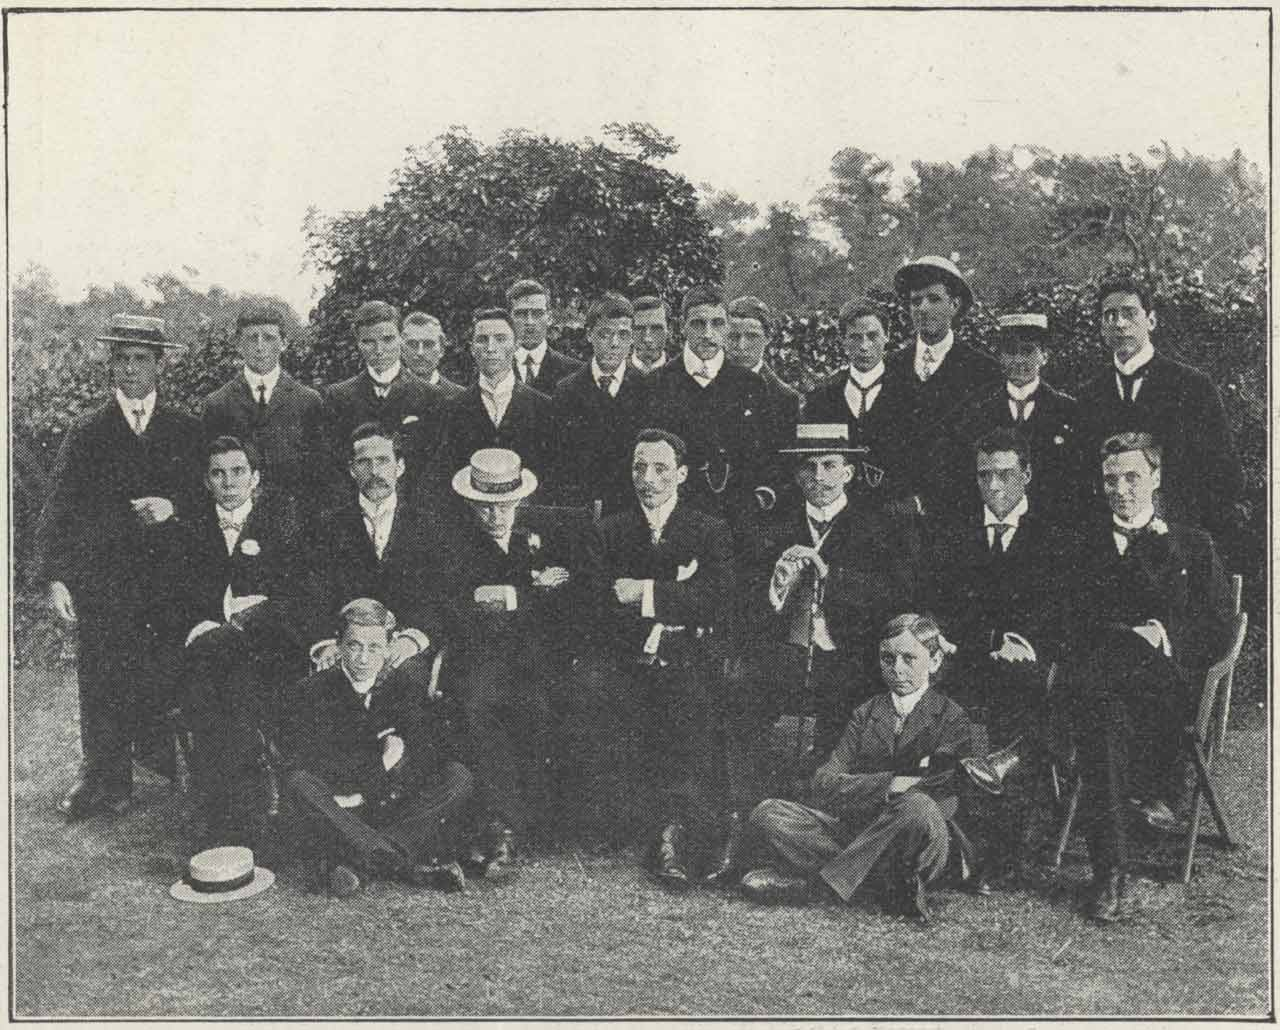
\includegraphics[width=\textwidth]{figures/photo/Greenwich-Observatory-computing-staff-1902.jpg}
      \end{figure}
    \end{column}
    
    \begin{column}{0.4\textwidth}
      \begin{itemize}
        \item Employed computers
        \item 13--20 years old
        \item no particularly strong background in mathematics
        \item A basic understanding of logarithms, algebra, etc\dots
      \end{itemize}
    \end{column}
    \end{columns}

\end{frame}


\begin{frame}{George Airy}
    Airy built complexity into the process, assigning \emph{human computers} 
    to calculate \& verify the \emph{right ascension} and \emph{declination} of stars.

    \begin{figure}
    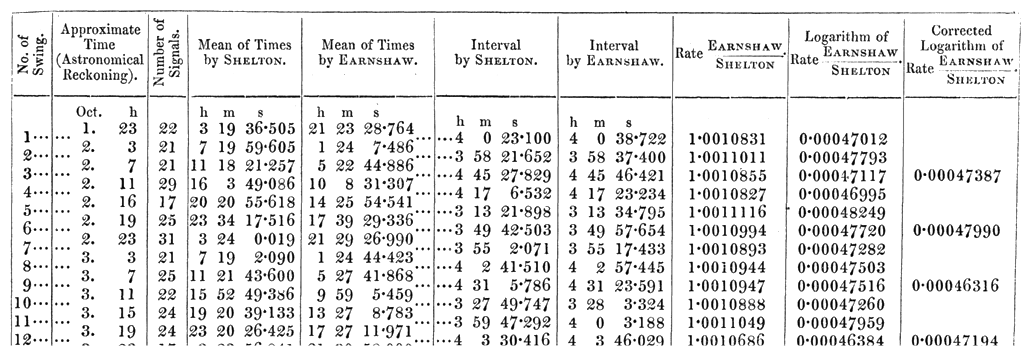
\includegraphics[width=\textwidth]{figures/complexity/pw_literature/airy.png}
    \end{figure}
\end{frame}


\subfile{piecework-simple}
\subfile{piecework-complex}


\begin{frame}{Comparisons}
\begin{itemize}
  \item Limited array of tasks versus arbitrarily complex work
  \begin{itemize}
    \item \emph{Building} planes versus \emph{fixing} trains
  \end{itemize}
  \item \normalsize{Has technology changed this?}
    \begin{itemize}
      \item Technology makes \emph{some} complex tasks relatively trivial
      \item Measuring workers is easier than ever
    \end{itemize}
\end{itemize}
\end{frame}

\begin{frame}{Complexity} % {Cab Drivers}
  \begin{figure}
  \includegraphics<1>[width=\textwidth]{figures/photo/knowledge-student.jpg}
  \only<2>{
  \begin{columns}
  \begin{column}{0.2\textwidth}
  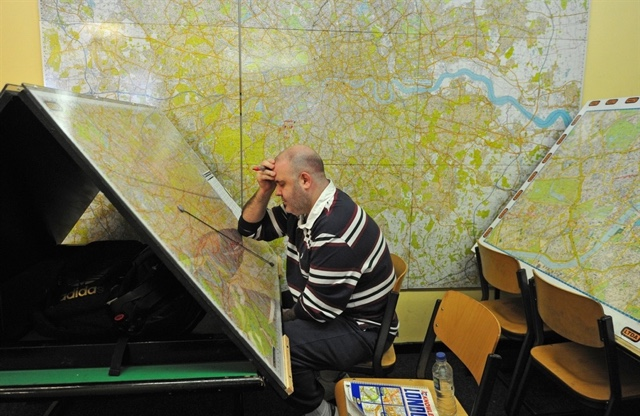
\includegraphics[width=\textwidth]{figures/photo/knowledge-student.jpg}
  \end{column}
  \begin{column}{0.8\textwidth}
  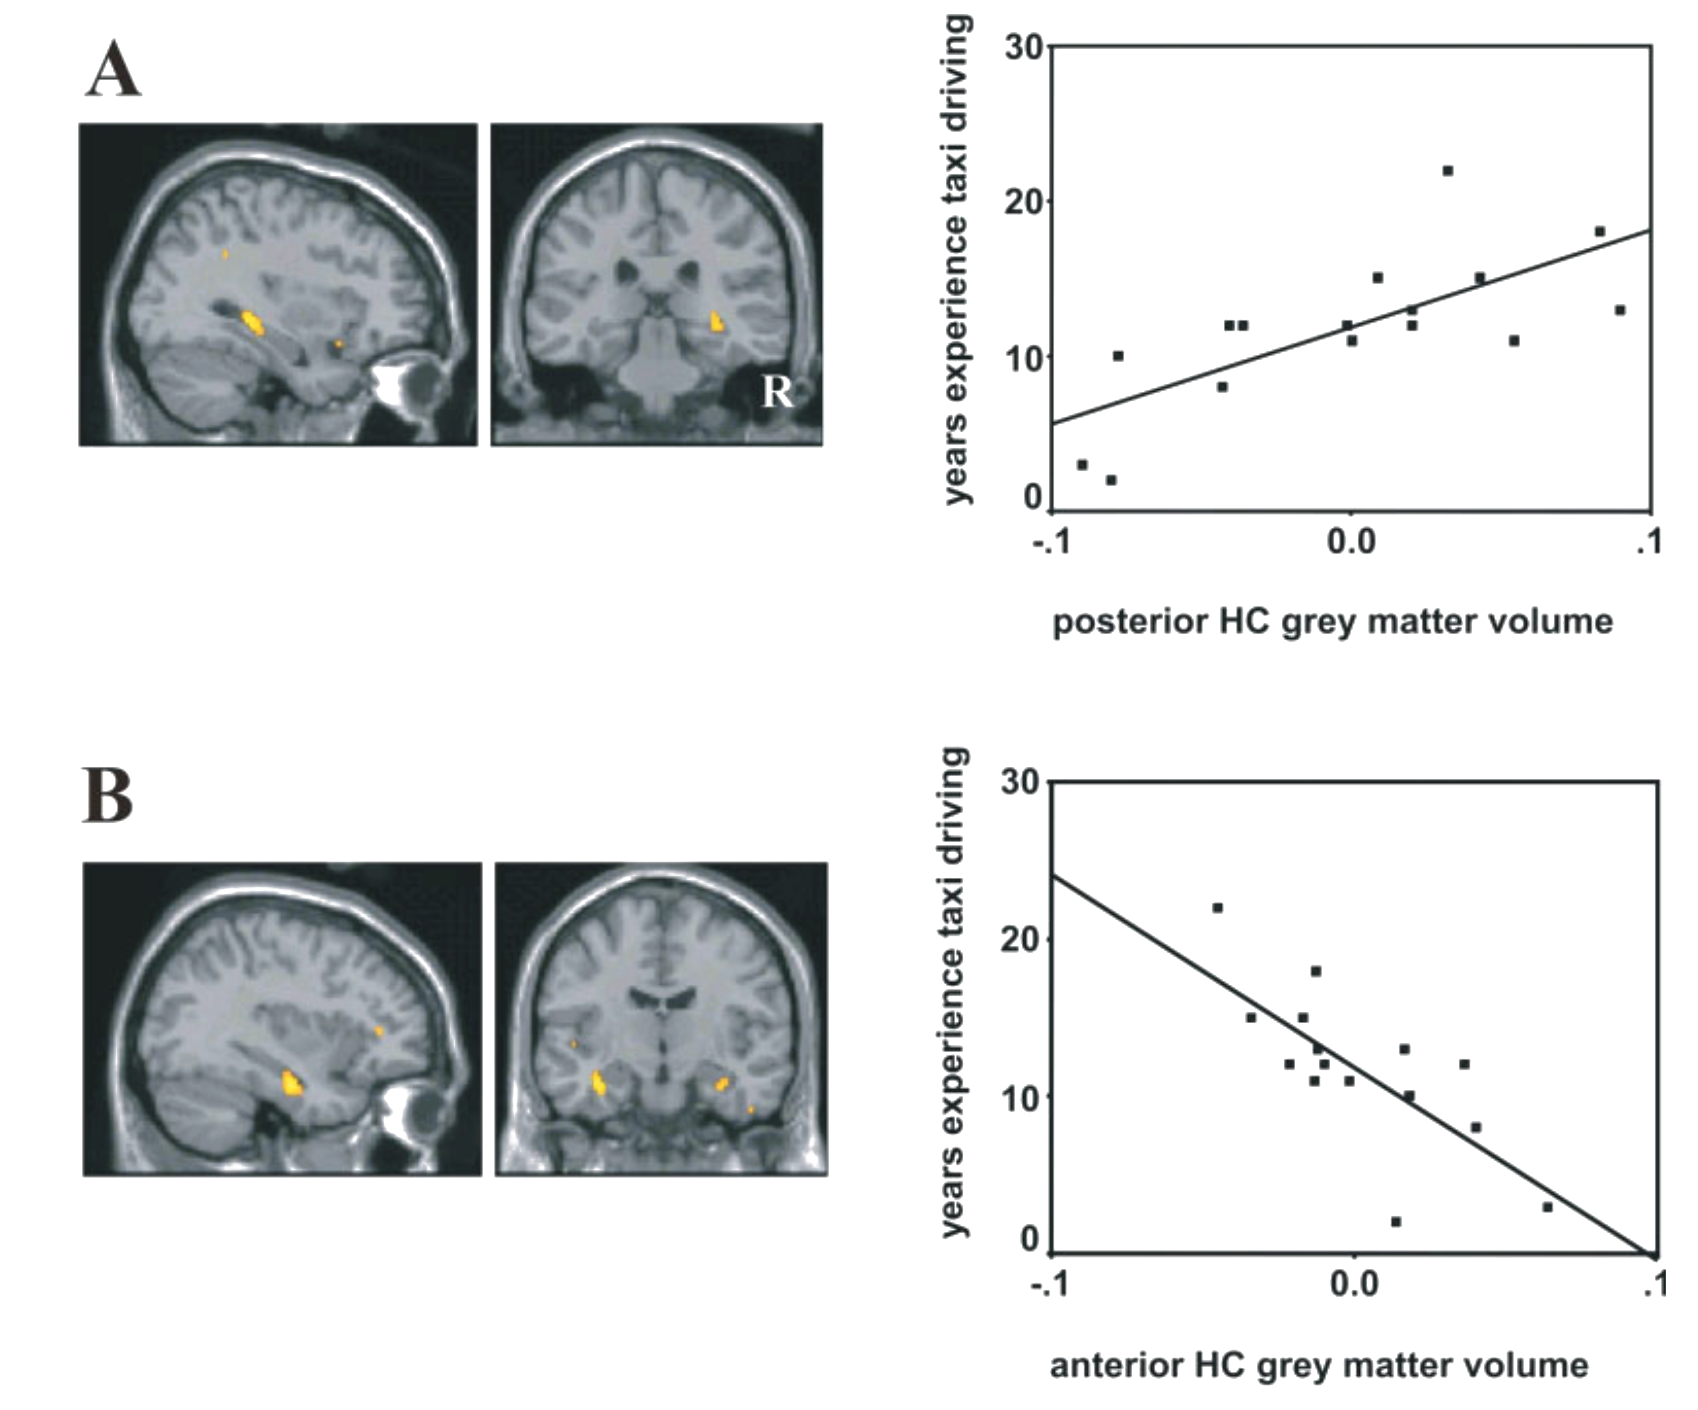
\includegraphics[width=\textwidth]{figures/complexity/brain_scans.png}
  \end{column}
  \end{columns}
  }
  \includegraphics<3>[width=\textwidth]{figures/photo/gps-map.jpg}
  \end{figure}
\end{frame}

\begin{frame}{Complexity} % {Algorithmic Measurement}
    notes
    \begin{itemize}
      \item I'm thinking of pointing to UpWork's screen recording tool as a way to measure workers
      \item also maybe google analytics and other ways of tracking web--based workers
    \end{itemize}
\end{frame}

\begin{frame}{Implications}
  \begin{itemize}
    \item We make stronger assumptions about workers' abilities thanks to technology
    \item Evaluation remains difficult, but we're trying to find stopgap solutions through decomposition
    \item We're still not solving the problems of inherently subjectively judged work
  \end{itemize}
\end{frame}

\onlyinsubfile{
  \printbibliography{}
}
\end{document}